% Options for packages loaded elsewhere
% Options for packages loaded elsewhere
\PassOptionsToPackage{unicode}{hyperref}
\PassOptionsToPackage{hyphens}{url}
\PassOptionsToPackage{dvipsnames,svgnames,x11names}{xcolor}
%
\documentclass[
  letterpaper,
  DIV=11,
  numbers=noendperiod]{scrartcl}
\usepackage{xcolor}
\usepackage{amsmath,amssymb}
\setcounter{secnumdepth}{-\maxdimen} % remove section numbering
\usepackage{iftex}
\ifPDFTeX
  \usepackage[T1]{fontenc}
  \usepackage[utf8]{inputenc}
  \usepackage{textcomp} % provide euro and other symbols
\else % if luatex or xetex
  \usepackage{unicode-math} % this also loads fontspec
  \defaultfontfeatures{Scale=MatchLowercase}
  \defaultfontfeatures[\rmfamily]{Ligatures=TeX,Scale=1}
\fi
\usepackage{lmodern}
\ifPDFTeX\else
  % xetex/luatex font selection
\fi
% Use upquote if available, for straight quotes in verbatim environments
\IfFileExists{upquote.sty}{\usepackage{upquote}}{}
\IfFileExists{microtype.sty}{% use microtype if available
  \usepackage[]{microtype}
  \UseMicrotypeSet[protrusion]{basicmath} % disable protrusion for tt fonts
}{}
\makeatletter
\@ifundefined{KOMAClassName}{% if non-KOMA class
  \IfFileExists{parskip.sty}{%
    \usepackage{parskip}
  }{% else
    \setlength{\parindent}{0pt}
    \setlength{\parskip}{6pt plus 2pt minus 1pt}}
}{% if KOMA class
  \KOMAoptions{parskip=half}}
\makeatother
% Make \paragraph and \subparagraph free-standing
\makeatletter
\ifx\paragraph\undefined\else
  \let\oldparagraph\paragraph
  \renewcommand{\paragraph}{
    \@ifstar
      \xxxParagraphStar
      \xxxParagraphNoStar
  }
  \newcommand{\xxxParagraphStar}[1]{\oldparagraph*{#1}\mbox{}}
  \newcommand{\xxxParagraphNoStar}[1]{\oldparagraph{#1}\mbox{}}
\fi
\ifx\subparagraph\undefined\else
  \let\oldsubparagraph\subparagraph
  \renewcommand{\subparagraph}{
    \@ifstar
      \xxxSubParagraphStar
      \xxxSubParagraphNoStar
  }
  \newcommand{\xxxSubParagraphStar}[1]{\oldsubparagraph*{#1}\mbox{}}
  \newcommand{\xxxSubParagraphNoStar}[1]{\oldsubparagraph{#1}\mbox{}}
\fi
\makeatother

\usepackage{color}
\usepackage{fancyvrb}
\newcommand{\VerbBar}{|}
\newcommand{\VERB}{\Verb[commandchars=\\\{\}]}
\DefineVerbatimEnvironment{Highlighting}{Verbatim}{commandchars=\\\{\}}
% Add ',fontsize=\small' for more characters per line
\usepackage{framed}
\definecolor{shadecolor}{RGB}{241,243,245}
\newenvironment{Shaded}{\begin{snugshade}}{\end{snugshade}}
\newcommand{\AlertTok}[1]{\textcolor[rgb]{0.68,0.00,0.00}{#1}}
\newcommand{\AnnotationTok}[1]{\textcolor[rgb]{0.37,0.37,0.37}{#1}}
\newcommand{\AttributeTok}[1]{\textcolor[rgb]{0.40,0.45,0.13}{#1}}
\newcommand{\BaseNTok}[1]{\textcolor[rgb]{0.68,0.00,0.00}{#1}}
\newcommand{\BuiltInTok}[1]{\textcolor[rgb]{0.00,0.23,0.31}{#1}}
\newcommand{\CharTok}[1]{\textcolor[rgb]{0.13,0.47,0.30}{#1}}
\newcommand{\CommentTok}[1]{\textcolor[rgb]{0.37,0.37,0.37}{#1}}
\newcommand{\CommentVarTok}[1]{\textcolor[rgb]{0.37,0.37,0.37}{\textit{#1}}}
\newcommand{\ConstantTok}[1]{\textcolor[rgb]{0.56,0.35,0.01}{#1}}
\newcommand{\ControlFlowTok}[1]{\textcolor[rgb]{0.00,0.23,0.31}{\textbf{#1}}}
\newcommand{\DataTypeTok}[1]{\textcolor[rgb]{0.68,0.00,0.00}{#1}}
\newcommand{\DecValTok}[1]{\textcolor[rgb]{0.68,0.00,0.00}{#1}}
\newcommand{\DocumentationTok}[1]{\textcolor[rgb]{0.37,0.37,0.37}{\textit{#1}}}
\newcommand{\ErrorTok}[1]{\textcolor[rgb]{0.68,0.00,0.00}{#1}}
\newcommand{\ExtensionTok}[1]{\textcolor[rgb]{0.00,0.23,0.31}{#1}}
\newcommand{\FloatTok}[1]{\textcolor[rgb]{0.68,0.00,0.00}{#1}}
\newcommand{\FunctionTok}[1]{\textcolor[rgb]{0.28,0.35,0.67}{#1}}
\newcommand{\ImportTok}[1]{\textcolor[rgb]{0.00,0.46,0.62}{#1}}
\newcommand{\InformationTok}[1]{\textcolor[rgb]{0.37,0.37,0.37}{#1}}
\newcommand{\KeywordTok}[1]{\textcolor[rgb]{0.00,0.23,0.31}{\textbf{#1}}}
\newcommand{\NormalTok}[1]{\textcolor[rgb]{0.00,0.23,0.31}{#1}}
\newcommand{\OperatorTok}[1]{\textcolor[rgb]{0.37,0.37,0.37}{#1}}
\newcommand{\OtherTok}[1]{\textcolor[rgb]{0.00,0.23,0.31}{#1}}
\newcommand{\PreprocessorTok}[1]{\textcolor[rgb]{0.68,0.00,0.00}{#1}}
\newcommand{\RegionMarkerTok}[1]{\textcolor[rgb]{0.00,0.23,0.31}{#1}}
\newcommand{\SpecialCharTok}[1]{\textcolor[rgb]{0.37,0.37,0.37}{#1}}
\newcommand{\SpecialStringTok}[1]{\textcolor[rgb]{0.13,0.47,0.30}{#1}}
\newcommand{\StringTok}[1]{\textcolor[rgb]{0.13,0.47,0.30}{#1}}
\newcommand{\VariableTok}[1]{\textcolor[rgb]{0.07,0.07,0.07}{#1}}
\newcommand{\VerbatimStringTok}[1]{\textcolor[rgb]{0.13,0.47,0.30}{#1}}
\newcommand{\WarningTok}[1]{\textcolor[rgb]{0.37,0.37,0.37}{\textit{#1}}}

\usepackage{longtable,booktabs,array}
\usepackage{calc} % for calculating minipage widths
% Correct order of tables after \paragraph or \subparagraph
\usepackage{etoolbox}
\makeatletter
\patchcmd\longtable{\par}{\if@noskipsec\mbox{}\fi\par}{}{}
\makeatother
% Allow footnotes in longtable head/foot
\IfFileExists{footnotehyper.sty}{\usepackage{footnotehyper}}{\usepackage{footnote}}
\makesavenoteenv{longtable}
\usepackage{graphicx}
\makeatletter
\newsavebox\pandoc@box
\newcommand*\pandocbounded[1]{% scales image to fit in text height/width
  \sbox\pandoc@box{#1}%
  \Gscale@div\@tempa{\textheight}{\dimexpr\ht\pandoc@box+\dp\pandoc@box\relax}%
  \Gscale@div\@tempb{\linewidth}{\wd\pandoc@box}%
  \ifdim\@tempb\p@<\@tempa\p@\let\@tempa\@tempb\fi% select the smaller of both
  \ifdim\@tempa\p@<\p@\scalebox{\@tempa}{\usebox\pandoc@box}%
  \else\usebox{\pandoc@box}%
  \fi%
}
% Set default figure placement to htbp
\def\fps@figure{htbp}
\makeatother





\setlength{\emergencystretch}{3em} % prevent overfull lines

\providecommand{\tightlist}{%
  \setlength{\itemsep}{0pt}\setlength{\parskip}{0pt}}



 


\usepackage{booktabs}
\usepackage{longtable}
\usepackage{array}
\usepackage{multirow}
\usepackage{wrapfig}
\usepackage{float}
\usepackage{colortbl}
\usepackage{pdflscape}
\usepackage{tabu}
\usepackage{threeparttable}
\usepackage{threeparttablex}
\usepackage[normalem]{ulem}
\usepackage{makecell}
\usepackage{xcolor}
\KOMAoption{captions}{tableheading}
\makeatletter
\@ifpackageloaded{caption}{}{\usepackage{caption}}
\AtBeginDocument{%
\ifdefined\contentsname
  \renewcommand*\contentsname{Table of contents}
\else
  \newcommand\contentsname{Table of contents}
\fi
\ifdefined\listfigurename
  \renewcommand*\listfigurename{List of Figures}
\else
  \newcommand\listfigurename{List of Figures}
\fi
\ifdefined\listtablename
  \renewcommand*\listtablename{List of Tables}
\else
  \newcommand\listtablename{List of Tables}
\fi
\ifdefined\figurename
  \renewcommand*\figurename{Figure}
\else
  \newcommand\figurename{Figure}
\fi
\ifdefined\tablename
  \renewcommand*\tablename{Table}
\else
  \newcommand\tablename{Table}
\fi
}
\@ifpackageloaded{float}{}{\usepackage{float}}
\floatstyle{ruled}
\@ifundefined{c@chapter}{\newfloat{codelisting}{h}{lop}}{\newfloat{codelisting}{h}{lop}[chapter]}
\floatname{codelisting}{Listing}
\newcommand*\listoflistings{\listof{codelisting}{List of Listings}}
\makeatother
\makeatletter
\makeatother
\makeatletter
\@ifpackageloaded{caption}{}{\usepackage{caption}}
\@ifpackageloaded{subcaption}{}{\usepackage{subcaption}}
\makeatother
\usepackage{bookmark}
\IfFileExists{xurl.sty}{\usepackage{xurl}}{} % add URL line breaks if available
\urlstyle{same}
\hypersetup{
  pdftitle={Synoptic LE: Manual Redox Probes},
  pdfauthor={Roberta Peixoto \& Fausto Machado-Silva},
  colorlinks=true,
  linkcolor={blue},
  filecolor={Maroon},
  citecolor={Blue},
  urlcolor={Blue},
  pdfcreator={LaTeX via pandoc}}


\title{Synoptic LE: Manual Redox Probes}
\author{Roberta Peixoto \& Fausto Machado-Silva}
\date{2026-09-01}
\begin{document}
\maketitle

\renewcommand*\contentsname{Table of contents}
{
\hypersetup{linkcolor=}
\setcounter{tocdepth}{3}
\tableofcontents
}

\section{Measurements taken with SWAP Redox Probes \& Calomel Ref
probe}\label{measurements-taken-with-swap-redox-probes-calomel-ref-probe}

\section{Protocol:
https://docs.google.com/document/d/}\label{protocol-httpsdocs.google.comdocumentd}

\section{1dL2ZPhLFBAZJmVBCfKxup\_KOYY96qA5IWfJmQen50pY/edit}\label{dl2zphlfbazjmvbcfkxup_koyy96qa5iwfjmqen50pyedit}

\section{Units = mV}\label{units-mv}

\#\#Add Required Packages

\#\#Setup

\begin{Shaded}
\begin{Highlighting}[]
\DocumentationTok{\#\#\#\#\#\# File Names {-} PLEASE CHANGE }
\CommentTok{\#file path and name for raw summary data file }
\NormalTok{dat }\OtherTok{\textless{}{-}} \FunctionTok{read.csv}\NormalTok{(}\StringTok{"Raw\_Data/COMPASS\_Synoptic\_LE\_Redox\_2022\_2025\_Raw.csv"}\NormalTok{)}
\CommentTok{\#soildat \textless{}{-} read.csv("Raw Data/LE\_Soil\_pH.csv") }

\DocumentationTok{\#\#Fix Sample Zone naming}
\NormalTok{dat }\OtherTok{\textless{}{-}}\NormalTok{ dat }\SpecialCharTok{\%\textgreater{}\%}
  \FunctionTok{mutate}\NormalTok{(}\AttributeTok{Zone =} \FunctionTok{ifelse}\NormalTok{(Zone }\SpecialCharTok{==} \StringTok{"WE"}\NormalTok{, }\StringTok{"WC"}\NormalTok{, Zone))}\SpecialCharTok{\%\textgreater{}\%}
  \FunctionTok{rename}\NormalTok{(}\AttributeTok{Depth=}\NormalTok{Depth\_cm)}

\DocumentationTok{\#\#Std error function}
\NormalTok{std.error }\OtherTok{\textless{}{-}} \ControlFlowTok{function}\NormalTok{ (x, }\AttributeTok{na.rm=}\ConstantTok{FALSE}\NormalTok{)\{}
  \FunctionTok{sqrt}\NormalTok{(}\FunctionTok{var}\NormalTok{(x, }\AttributeTok{na.rm =}\NormalTok{ na.rm) }\SpecialCharTok{/} \FunctionTok{sum}\NormalTok{(}\SpecialCharTok{!}\FunctionTok{is.na}\NormalTok{(x)))\}}
\end{Highlighting}
\end{Shaded}

\subsection{Adjust Raw Readings by pH}\label{adjust-raw-readings-by-ph}

\subsection{Need to adjust for pH:}\label{need-to-adjust-for-ph}

\section{redox = redoxi + {[}(ph - 5)59 + 224{]} This is the equation
from
Megonigal,}\label{redox-redoxi-ph---559-224-this-is-the-equation-from-megonigal}

\section{Patrick, \& Faulkner 1993}\label{patrick-faulkner-1993}

\section{They used a calomel electrode and used 224 to adjust to
H2,}\label{they-used-a-calomel-electrode-and-used-224-to-adjust-to-h2}

\section{we use a KCl ref probe, so we need to add 202
instead}\label{we-use-a-kcl-ref-probe-so-we-need-to-add-202-instead}

\begin{Shaded}
\begin{Highlighting}[]
\DocumentationTok{\#\#Remove unnecessary column in redox data}
\NormalTok{prelong }\OtherTok{\textless{}{-}}\NormalTok{ dat }\SpecialCharTok{\%\textgreater{}\%} 
  \FunctionTok{select}\NormalTok{ (}\FunctionTok{c}\NormalTok{(}\DecValTok{1}\SpecialCharTok{:}\DecValTok{11}\NormalTok{), }\SpecialCharTok{{-}}\FunctionTok{c}\NormalTok{(}\StringTok{"Campaign"}\NormalTok{,}\StringTok{"Time"}\NormalTok{, }\StringTok{"Day"}\NormalTok{))}\SpecialCharTok{\%\textgreater{}\%} 
  \FunctionTok{mutate}\NormalTok{(}\AttributeTok{Notes =} \ConstantTok{NA}\NormalTok{, }
         \AttributeTok{Time\_24hr =} \ConstantTok{NA}\NormalTok{, }
         \AttributeTok{Time\_Zone =} \ConstantTok{NA}\NormalTok{, }
         \AttributeTok{Topography =} \ConstantTok{NA}\NormalTok{)}

\CommentTok{\#switch redox data to long format }
\NormalTok{datlong }\OtherTok{\textless{}{-}}  \FunctionTok{as.data.frame}\NormalTok{(}\FunctionTok{melt}\NormalTok{(}\FunctionTok{setDT}\NormalTok{(prelong), }\AttributeTok{id.vars =} \FunctionTok{c}\NormalTok{(}\StringTok{"Date"}\NormalTok{, }\StringTok{"Month"}\NormalTok{, }\StringTok{"Year"}\NormalTok{, }\StringTok{"Site"}\NormalTok{, }\StringTok{"Zone"}\NormalTok{, }\StringTok{"Depth"}\NormalTok{, }\StringTok{"Time\_24hr"}\NormalTok{, }\StringTok{"Time\_Zone"}\NormalTok{, }\StringTok{"Topography"}\NormalTok{, }\StringTok{"Notes"}\NormalTok{), }
                               \AttributeTok{variable.name =} \StringTok{"RP\_mV"}\NormalTok{))}

\CommentTok{\# \#\#Add in soil pH data}
\CommentTok{\# all\_corr \textless{}{-} merge(datlong, soildat, by = c("Site", "Zone"), all = TRUE)}
\CommentTok{\# }
\CommentTok{\# \#\#Adjust redox for pH}
\CommentTok{\# all\_corr \textless{}{-} all\_corr \%\textgreater{}\% }
\CommentTok{\#   mutate(value\_corr = value + ((pH {-} 5)*59 + 202))}

\DocumentationTok{\#\#Adjust redox for KCl ref probe}
\NormalTok{datlong }\OtherTok{\textless{}{-}}\NormalTok{ datlong }\SpecialCharTok{\%\textgreater{}\%}
  \FunctionTok{mutate}\NormalTok{(}\AttributeTok{value =} \FunctionTok{as.numeric}\NormalTok{(value),}
         \AttributeTok{value\_corr =}\NormalTok{ value }\SpecialCharTok{+} \DecValTok{202}\NormalTok{)}

\DocumentationTok{\#\#Average across all 5{-}6 measurements for each sampling Site, Zone, Depth, Month, Year}
\NormalTok{red1 }\OtherTok{\textless{}{-}}\NormalTok{ datlong }\SpecialCharTok{\%\textgreater{}\%}
  \FunctionTok{group\_by}\NormalTok{(Date, Month, Year, Site, Zone, Depth, Time\_24hr, Time\_Zone, Topography, Notes) }\SpecialCharTok{\%\textgreater{}\%}
  \FunctionTok{summarise}\NormalTok{(}\AttributeTok{Date =} \FunctionTok{first}\NormalTok{(Date), }
            \AttributeTok{Avg\_mV =} \FunctionTok{mean}\NormalTok{(value\_corr, }\AttributeTok{na.rm=}\ConstantTok{TRUE}\NormalTok{), }
            \AttributeTok{Std\_dv =} \FunctionTok{sd}\NormalTok{(value\_corr, }\AttributeTok{na.rm=}\ConstantTok{TRUE}\NormalTok{), }
            \AttributeTok{Std\_err =} \FunctionTok{std.error}\NormalTok{(value\_corr, }\AttributeTok{na.rm=}\ConstantTok{TRUE}\NormalTok{), }
            \AttributeTok{Notes =} \FunctionTok{first}\NormalTok{(Notes)}
\NormalTok{            )}

\CommentTok{\# head(red1)}
\end{Highlighting}
\end{Shaded}

\#\#Write Out Adjusted \& Avg'd Data

\subsection{Vizualize Data}\label{vizualize-data}

\pandocbounded{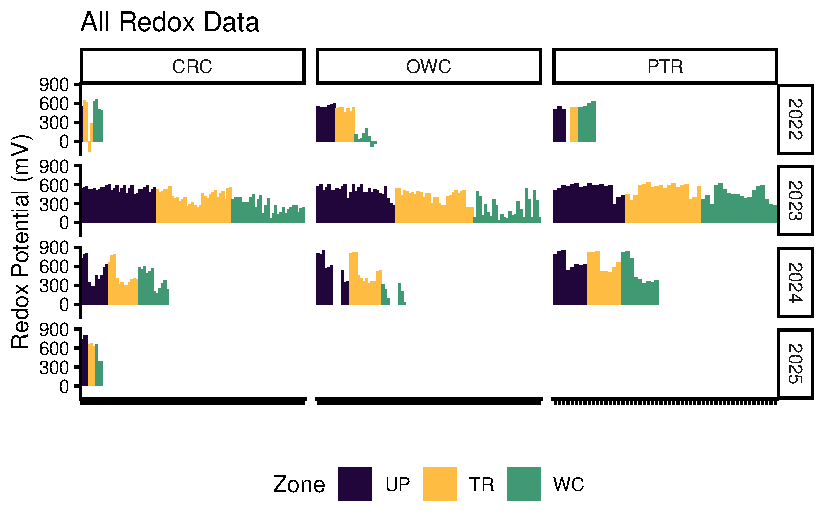
\includegraphics[keepaspectratio]{COMPASS_Synoptic_LE_Redox_Data_Processing_2022-2025_files/figure-pdf/visualize data-1.pdf}}

\pandocbounded{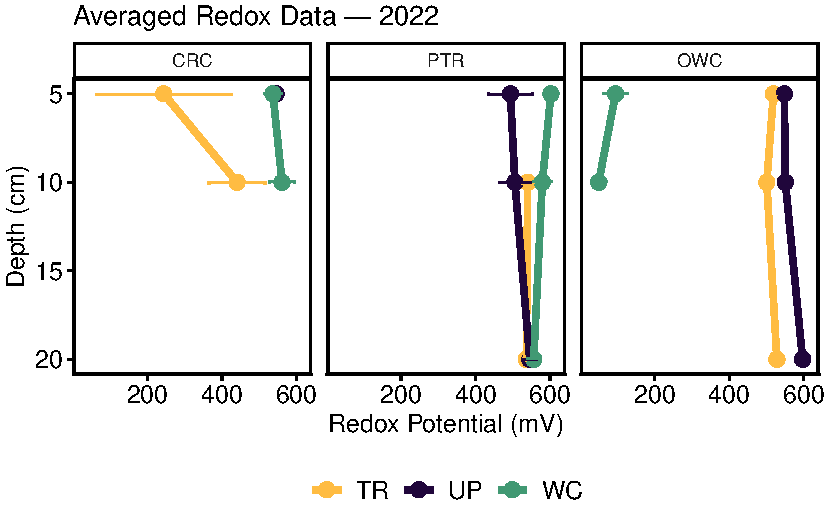
\includegraphics[keepaspectratio]{COMPASS_Synoptic_LE_Redox_Data_Processing_2022-2025_files/figure-pdf/visualize data-2.pdf}}

\pandocbounded{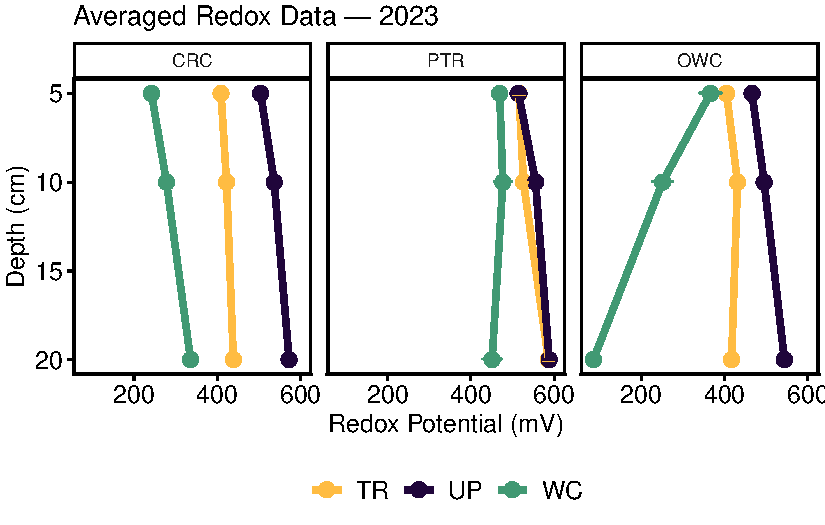
\includegraphics[keepaspectratio]{COMPASS_Synoptic_LE_Redox_Data_Processing_2022-2025_files/figure-pdf/visualize data-3.pdf}}

\pandocbounded{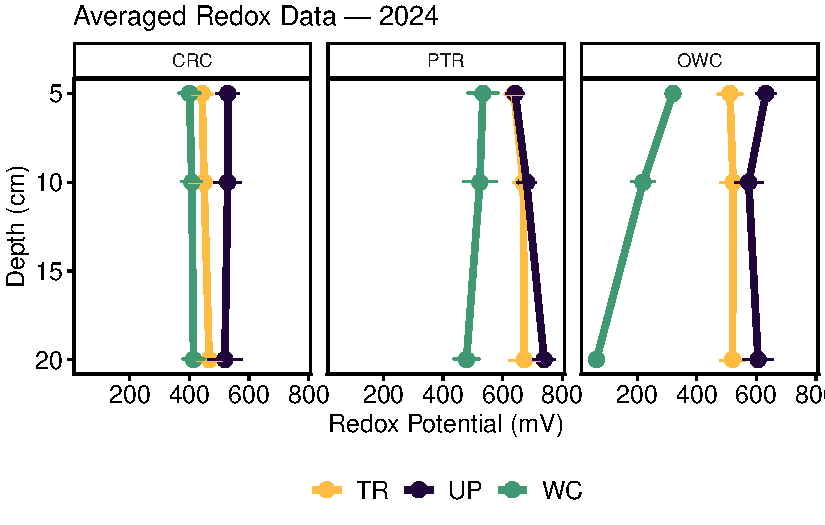
\includegraphics[keepaspectratio]{COMPASS_Synoptic_LE_Redox_Data_Processing_2022-2025_files/figure-pdf/visualize data-4.pdf}}

\pandocbounded{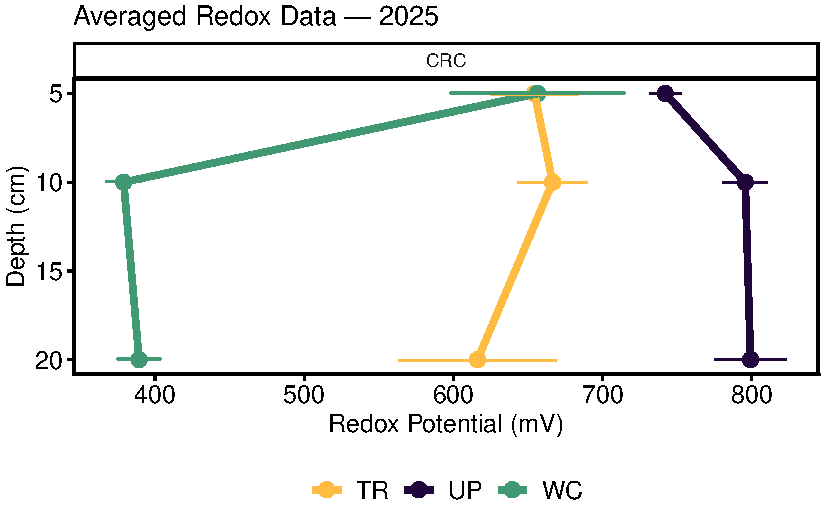
\includegraphics[keepaspectratio]{COMPASS_Synoptic_LE_Redox_Data_Processing_2022-2025_files/figure-pdf/visualize data-5.pdf}}

\subsection{Summarized data for Site and
Zone}\label{summarized-data-for-site-and-zone}

\pandocbounded{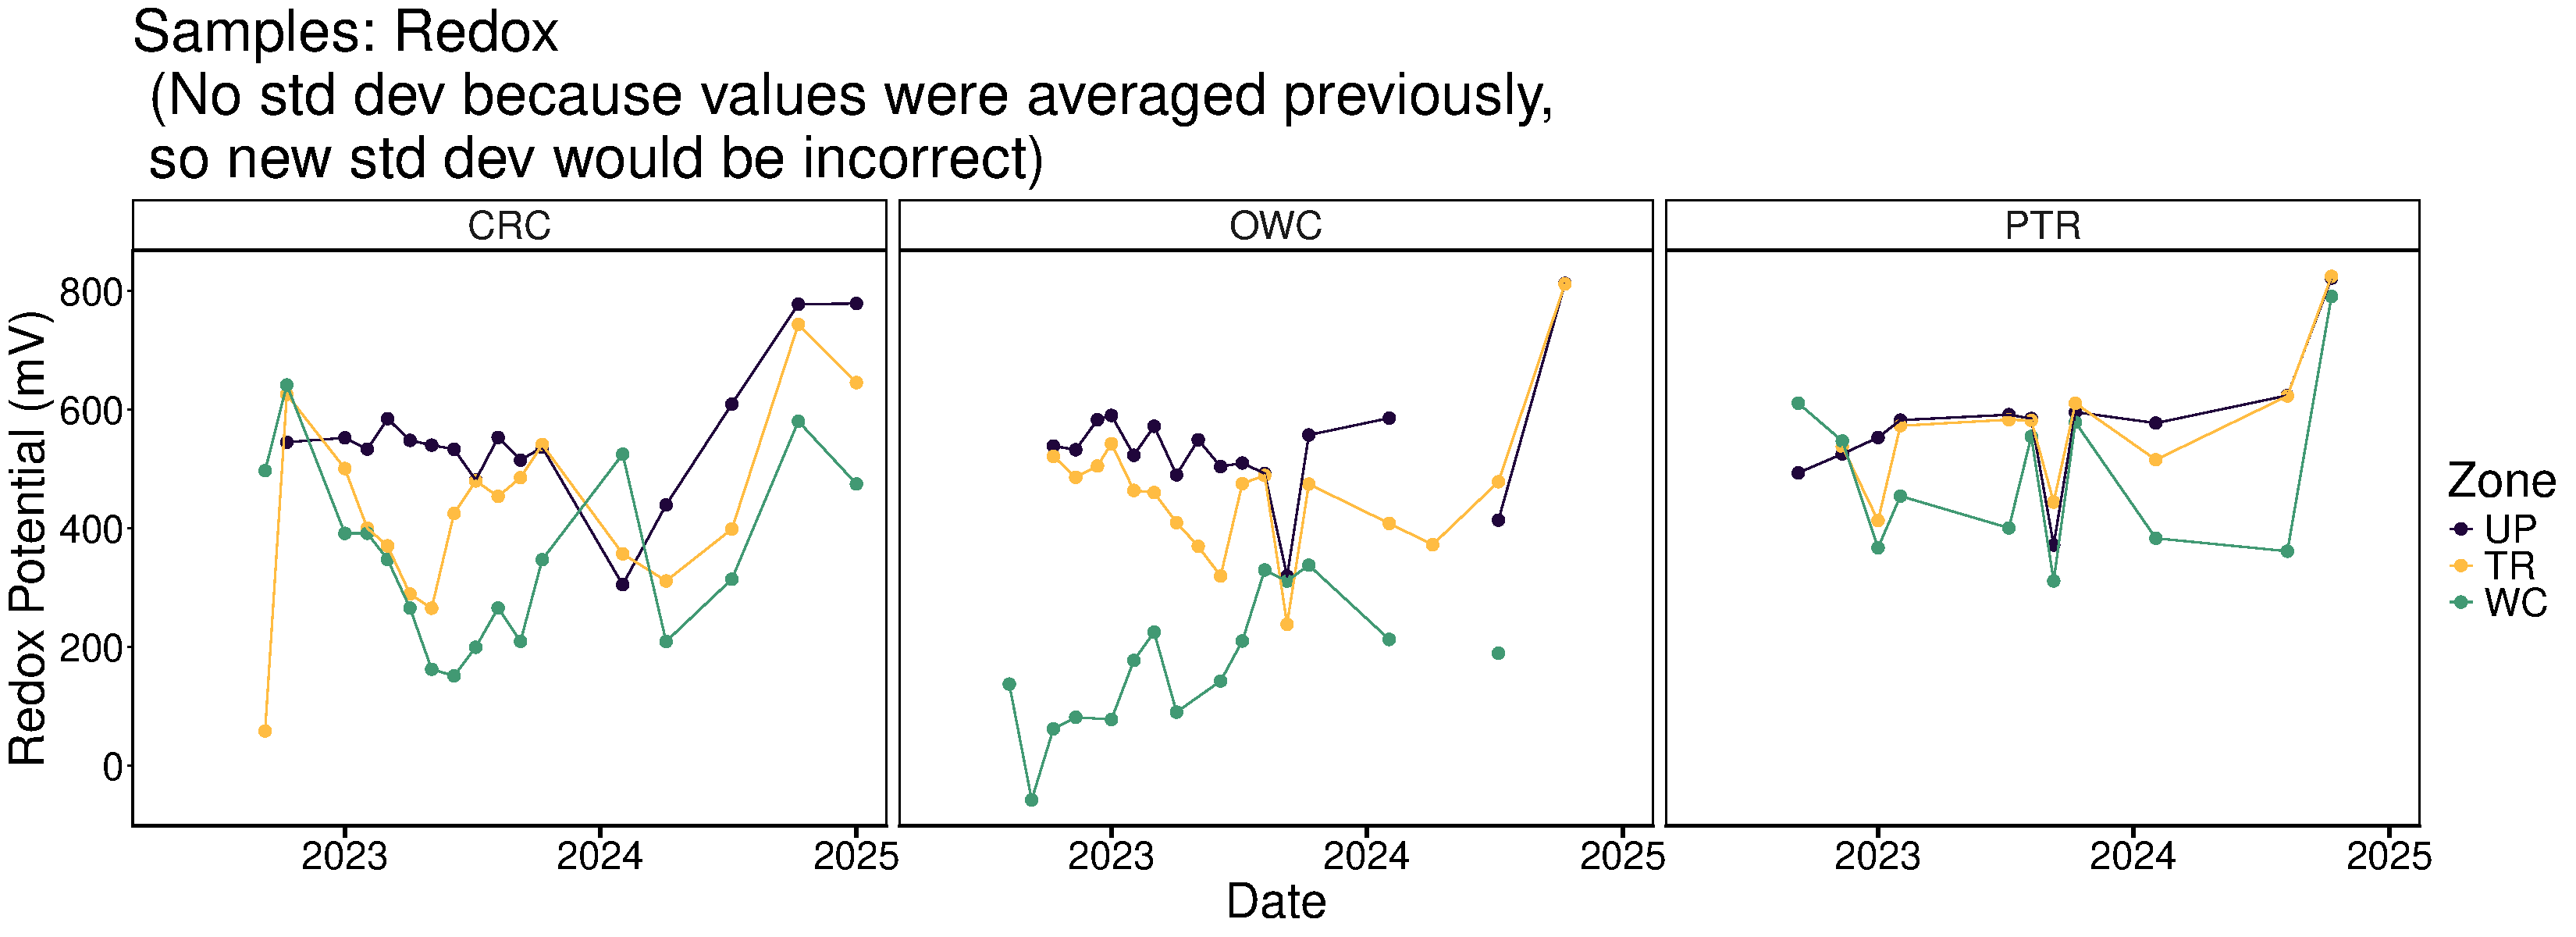
\includegraphics[keepaspectratio]{COMPASS_Synoptic_LE_Redox_Data_Processing_2022-2025_files/figure-pdf/Summarize and Visualize Data-1.pdf}}

\subsection{Summarized Data by Depth}\label{summarized-data-by-depth}

\pandocbounded{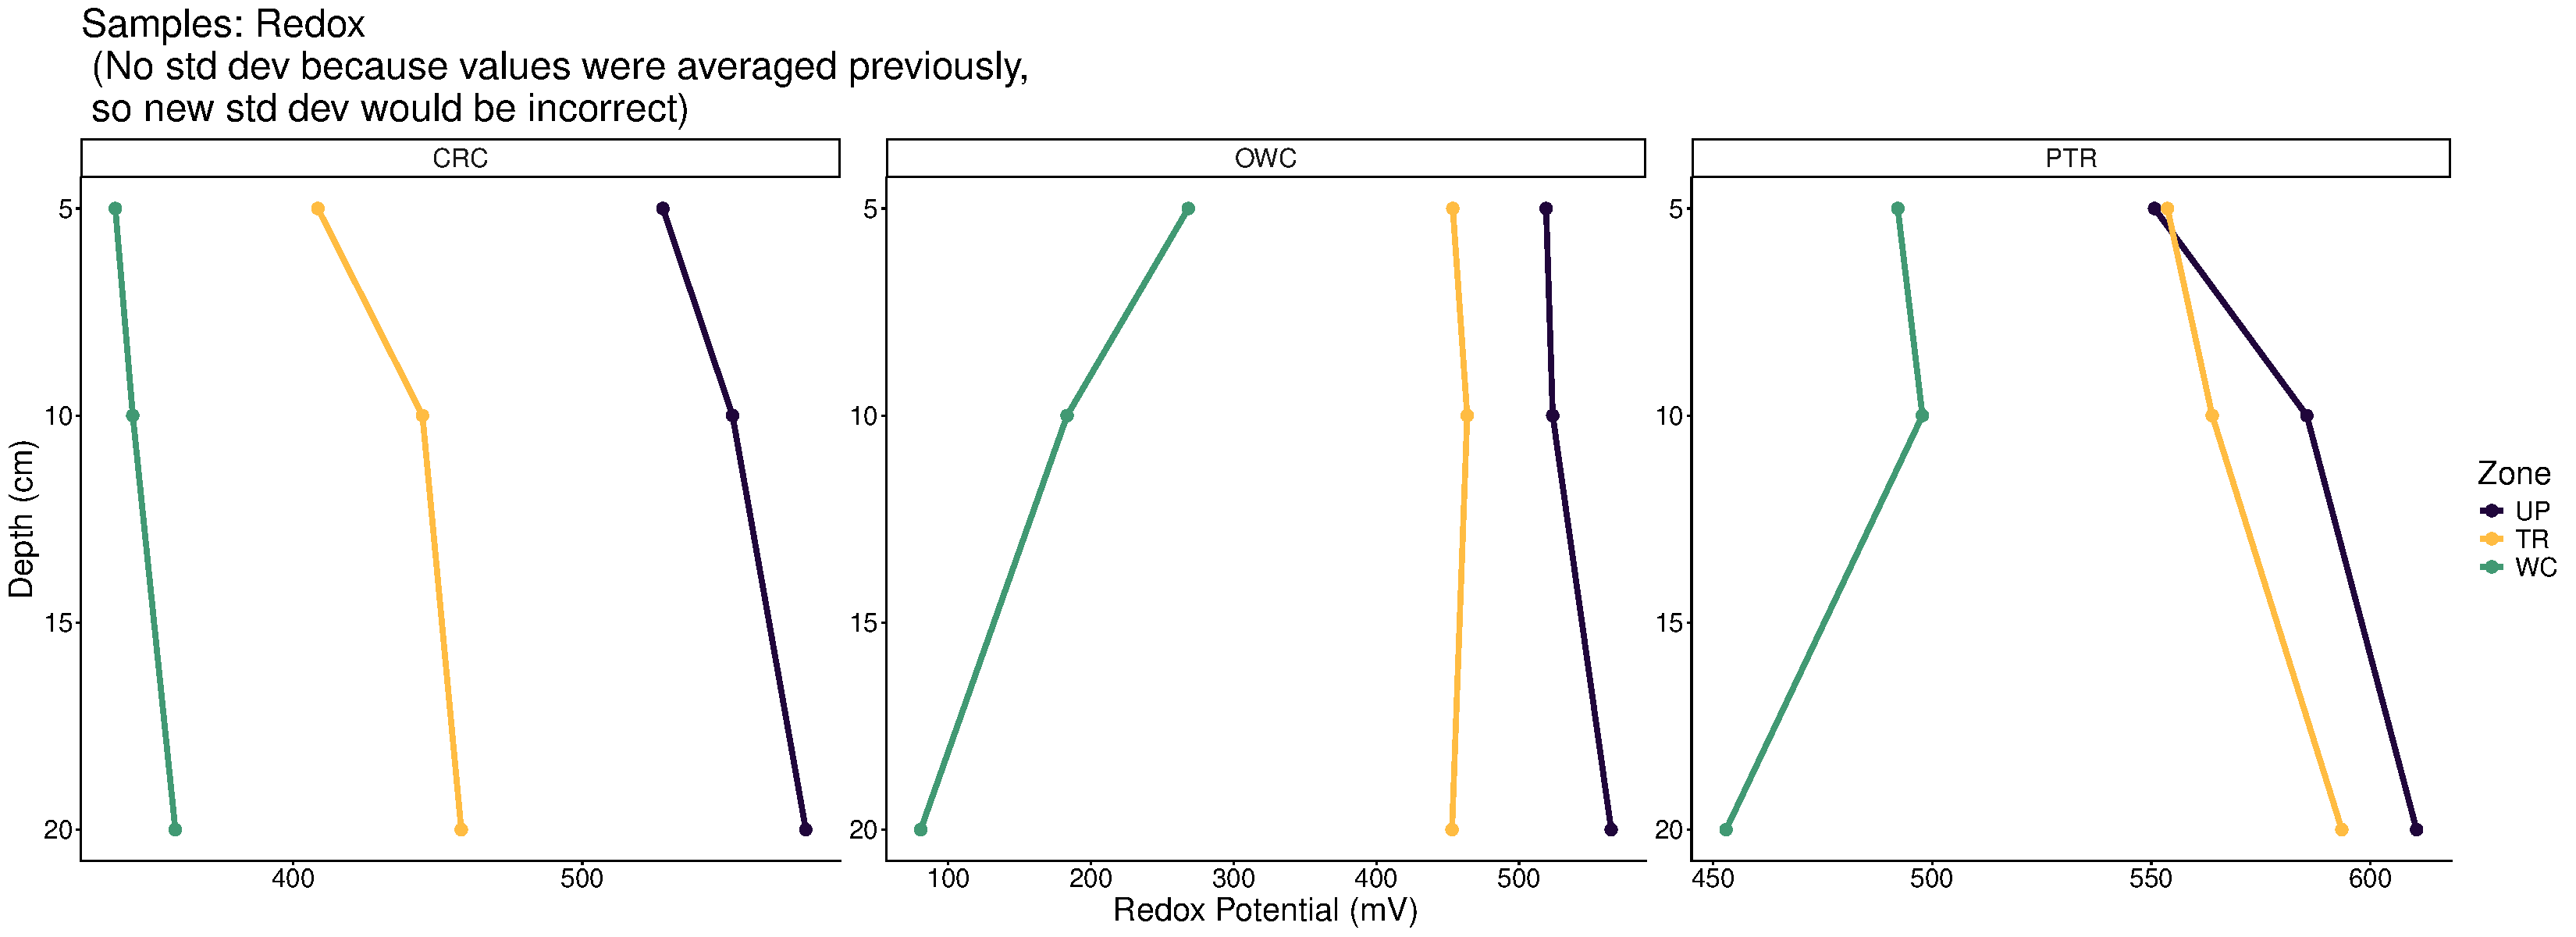
\includegraphics[keepaspectratio]{COMPASS_Synoptic_LE_Redox_Data_Processing_2022-2025_files/figure-pdf/Summarize Data by Depth-1.pdf}}

\subsection{Boxplot by depth}\label{boxplot-by-depth}

\pandocbounded{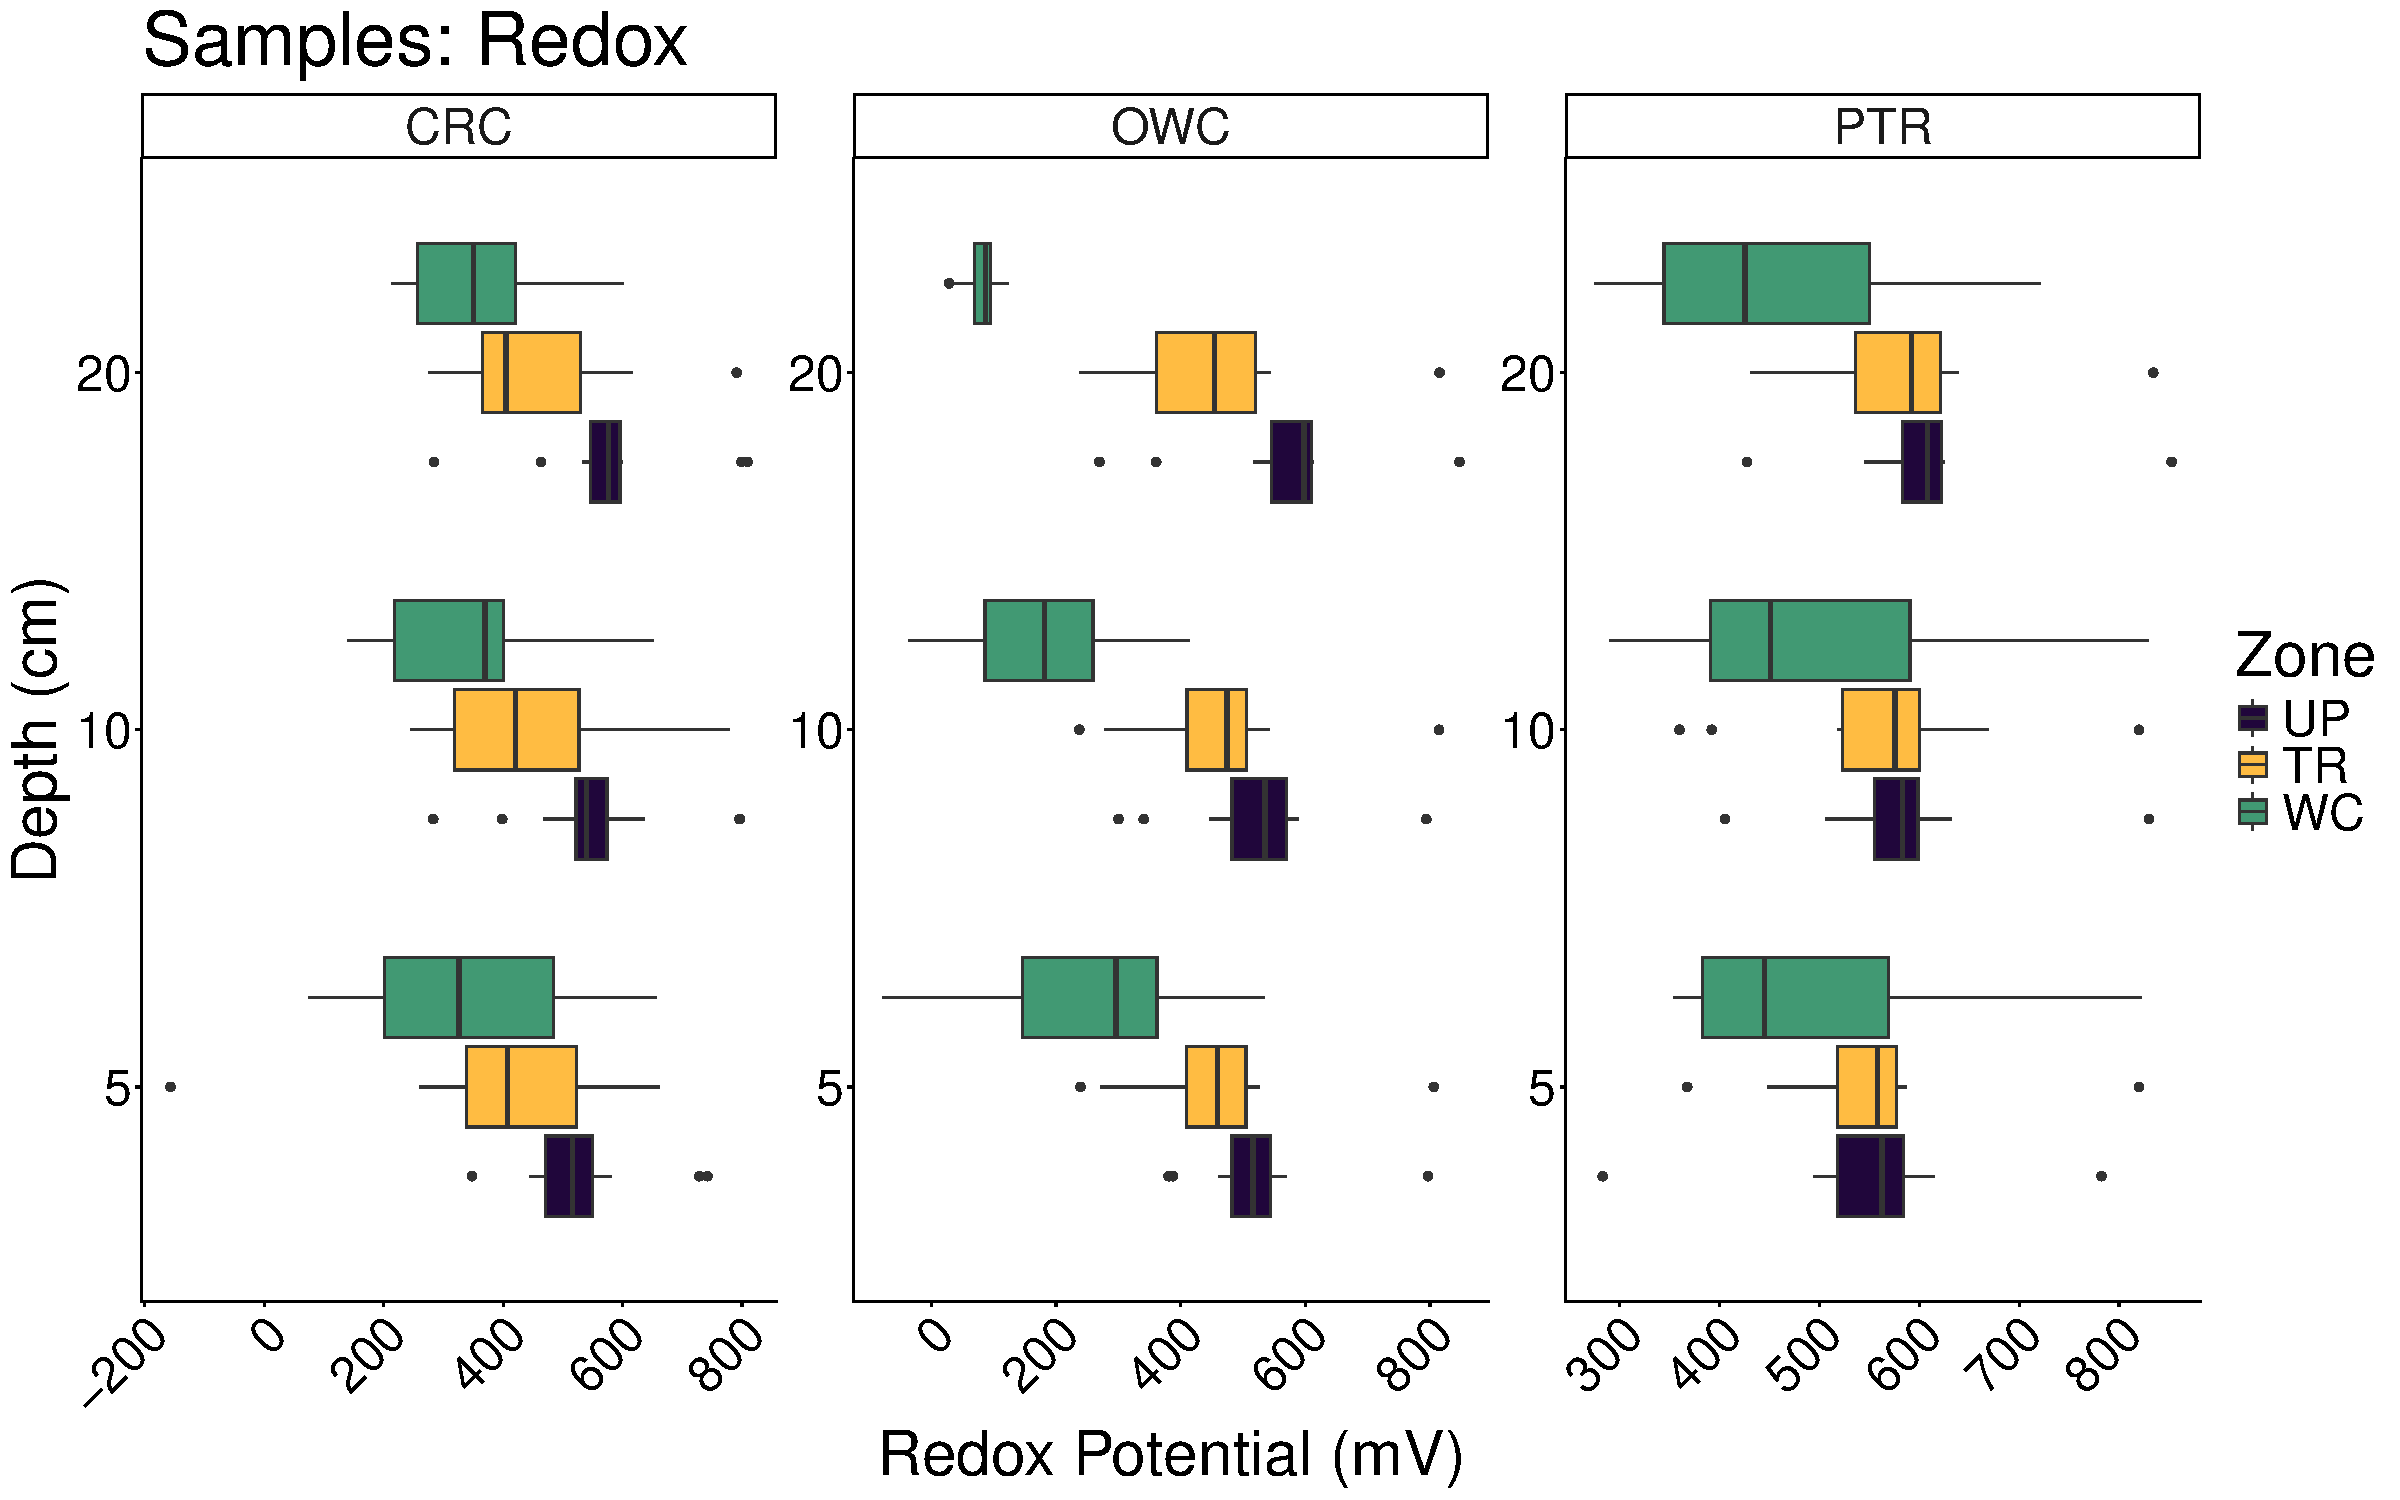
\includegraphics[keepaspectratio]{COMPASS_Synoptic_LE_Redox_Data_Processing_2022-2025_files/figure-pdf/Boxplot by depth-1.pdf}}

\subsection{Boxplot summary}\label{boxplot-summary}

\pandocbounded{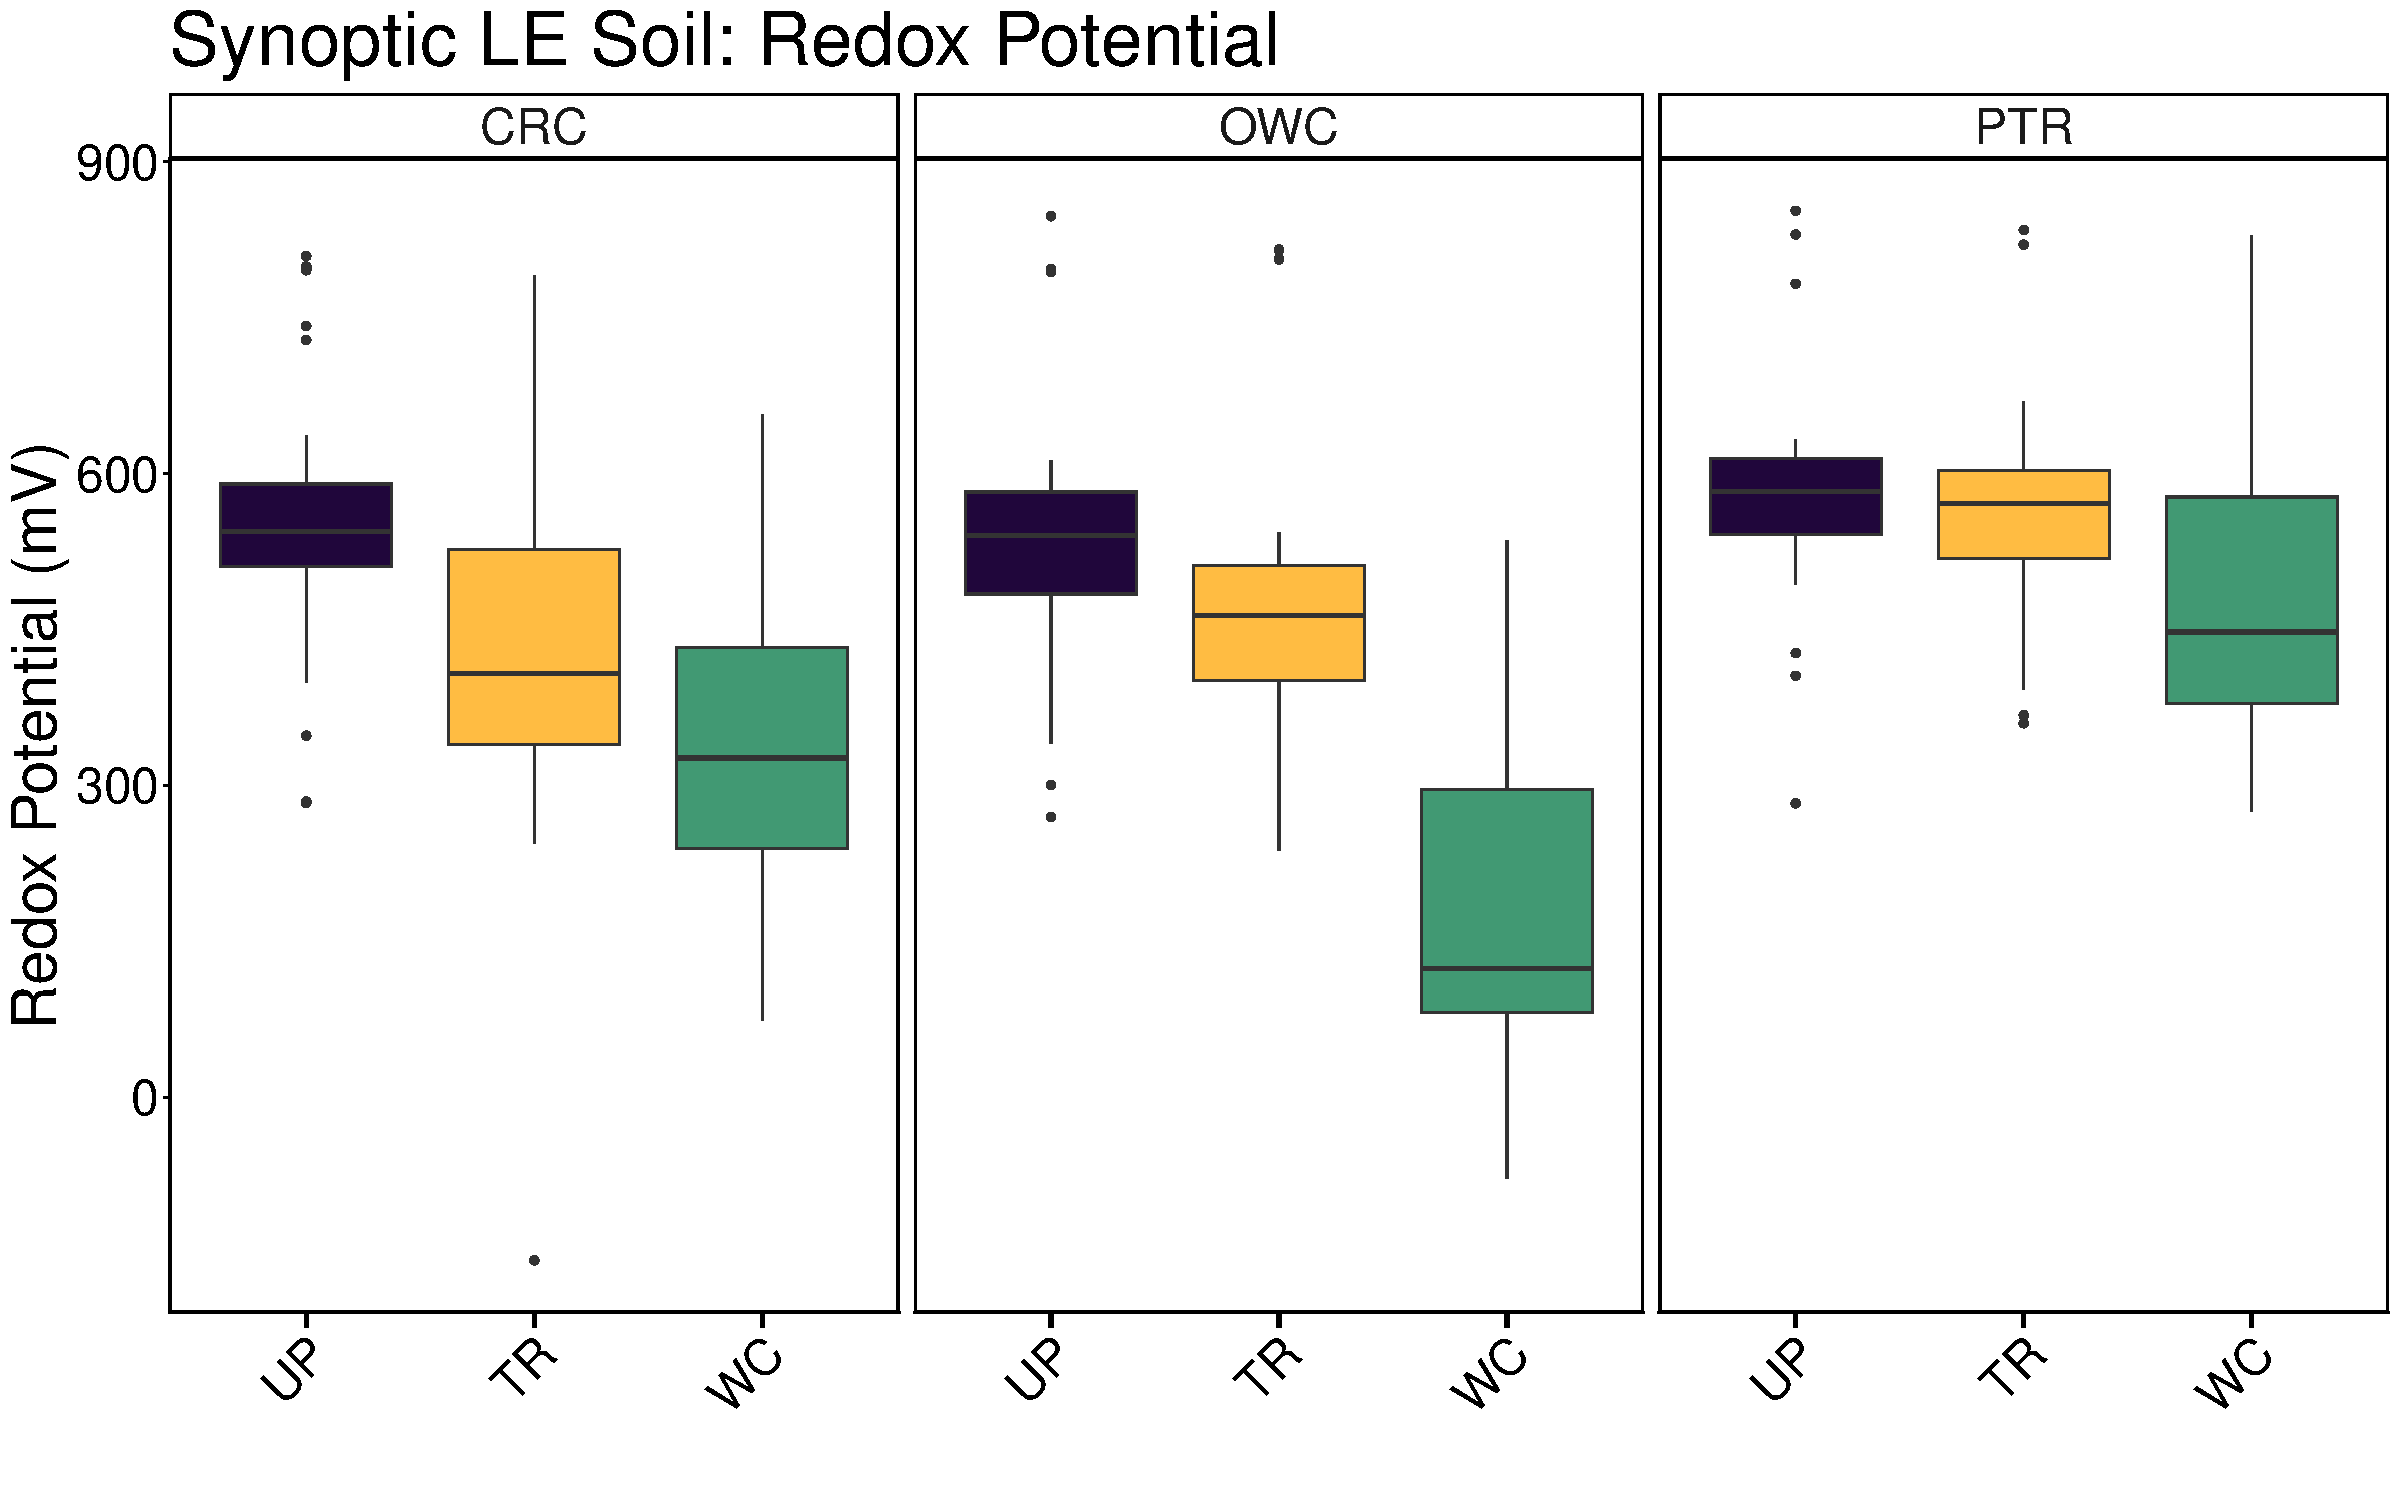
\includegraphics[keepaspectratio]{COMPASS_Synoptic_LE_Redox_Data_Processing_2022-2025_files/figure-pdf/Overall Boxplot-1.pdf}}

\begin{verbatim}
pdf 
  2 
\end{verbatim}

\#\#Calculate summary metrics

\#\#Calculate number of samples

\subsection{Summary Tables}\label{summary-tables}

\begin{table}[!h]
\centering
\caption{\label{tab:Summary table metrics}Summary Statistics}
\centering
\fontsize{12}{14}\selectfont
\begin{tabular}[t]{>{\raggedright\arraybackslash}p{0.8in}>{\raggedright\arraybackslash}p{1.6in}>{\raggedleft\arraybackslash}p{0.9in}>{\raggedleft\arraybackslash}p{0.9in}>{\raggedleft\arraybackslash}p{0.9in}}
\toprule
\textbf{Site} & \textbf{Plot} & \textbf{Min (mV)} & \textbf{Max (mV)} & \textbf{Mean (mV)}\\
\midrule
\textbf{\cellcolor{gray!10}{CRC}} & \cellcolor{gray!10}{TR} & \cellcolor{gray!10}{-156.97} & \cellcolor{gray!10}{790.95} & \cellcolor{gray!10}{436.25}\\
\textbf{CRC} & UP & 283.05 & 809.15 & 551.27\\
\textbf{\cellcolor{gray!10}{CRC}} & \cellcolor{gray!10}{WC} & \cellcolor{gray!10}{73.90} & \cellcolor{gray!10}{656.37} & \cellcolor{gray!10}{346.64}\\
\textbf{OWC} & TR & 237.53 & 815.43 & 457.00\\
\textbf{\cellcolor{gray!10}{OWC}} & \cellcolor{gray!10}{UP} & \cellcolor{gray!10}{269.65} & \cellcolor{gray!10}{847.57} & \cellcolor{gray!10}{534.83}\\
\addlinespace
\textbf{OWC} & WC & -78.30 & 535.33 & 184.81\\
\textbf{\cellcolor{gray!10}{PTR}} & \cellcolor{gray!10}{TR} & \cellcolor{gray!10}{359.80} & \cellcolor{gray!10}{834.32} & \cellcolor{gray!10}{570.12}\\
\textbf{PTR} & UP & 282.80 & 852.77 & 580.22\\
\textbf{\cellcolor{gray!10}{PTR}} & \cellcolor{gray!10}{WC} & \cellcolor{gray!10}{274.73} & \cellcolor{gray!10}{829.18} & \cellcolor{gray!10}{481.52}\\
\bottomrule
\end{tabular}
\end{table}

\subsection{Number of Samples}\label{number-of-samples}

\begin{table}[!h]
\centering
\caption{\label{tab:number of samples tables}Total Samples: 368}
\centering
\resizebox{\ifdim\width>\linewidth\linewidth\else\width\fi}{!}{
\fontsize{12}{14}\selectfont
\begin{tabular}[t]{>{}rr}
\toprule
\textbf{Year} & \textbf{Number\_of\_samples}\\
\midrule
\textbf{\cellcolor{gray!10}{2022}} & \cellcolor{gray!10}{41}\\
\textbf{2023} & 225\\
\textbf{\cellcolor{gray!10}{2024}} & \cellcolor{gray!10}{93}\\
\textbf{2025} & 9\\
\bottomrule
\end{tabular}}
\end{table}

\pandocbounded{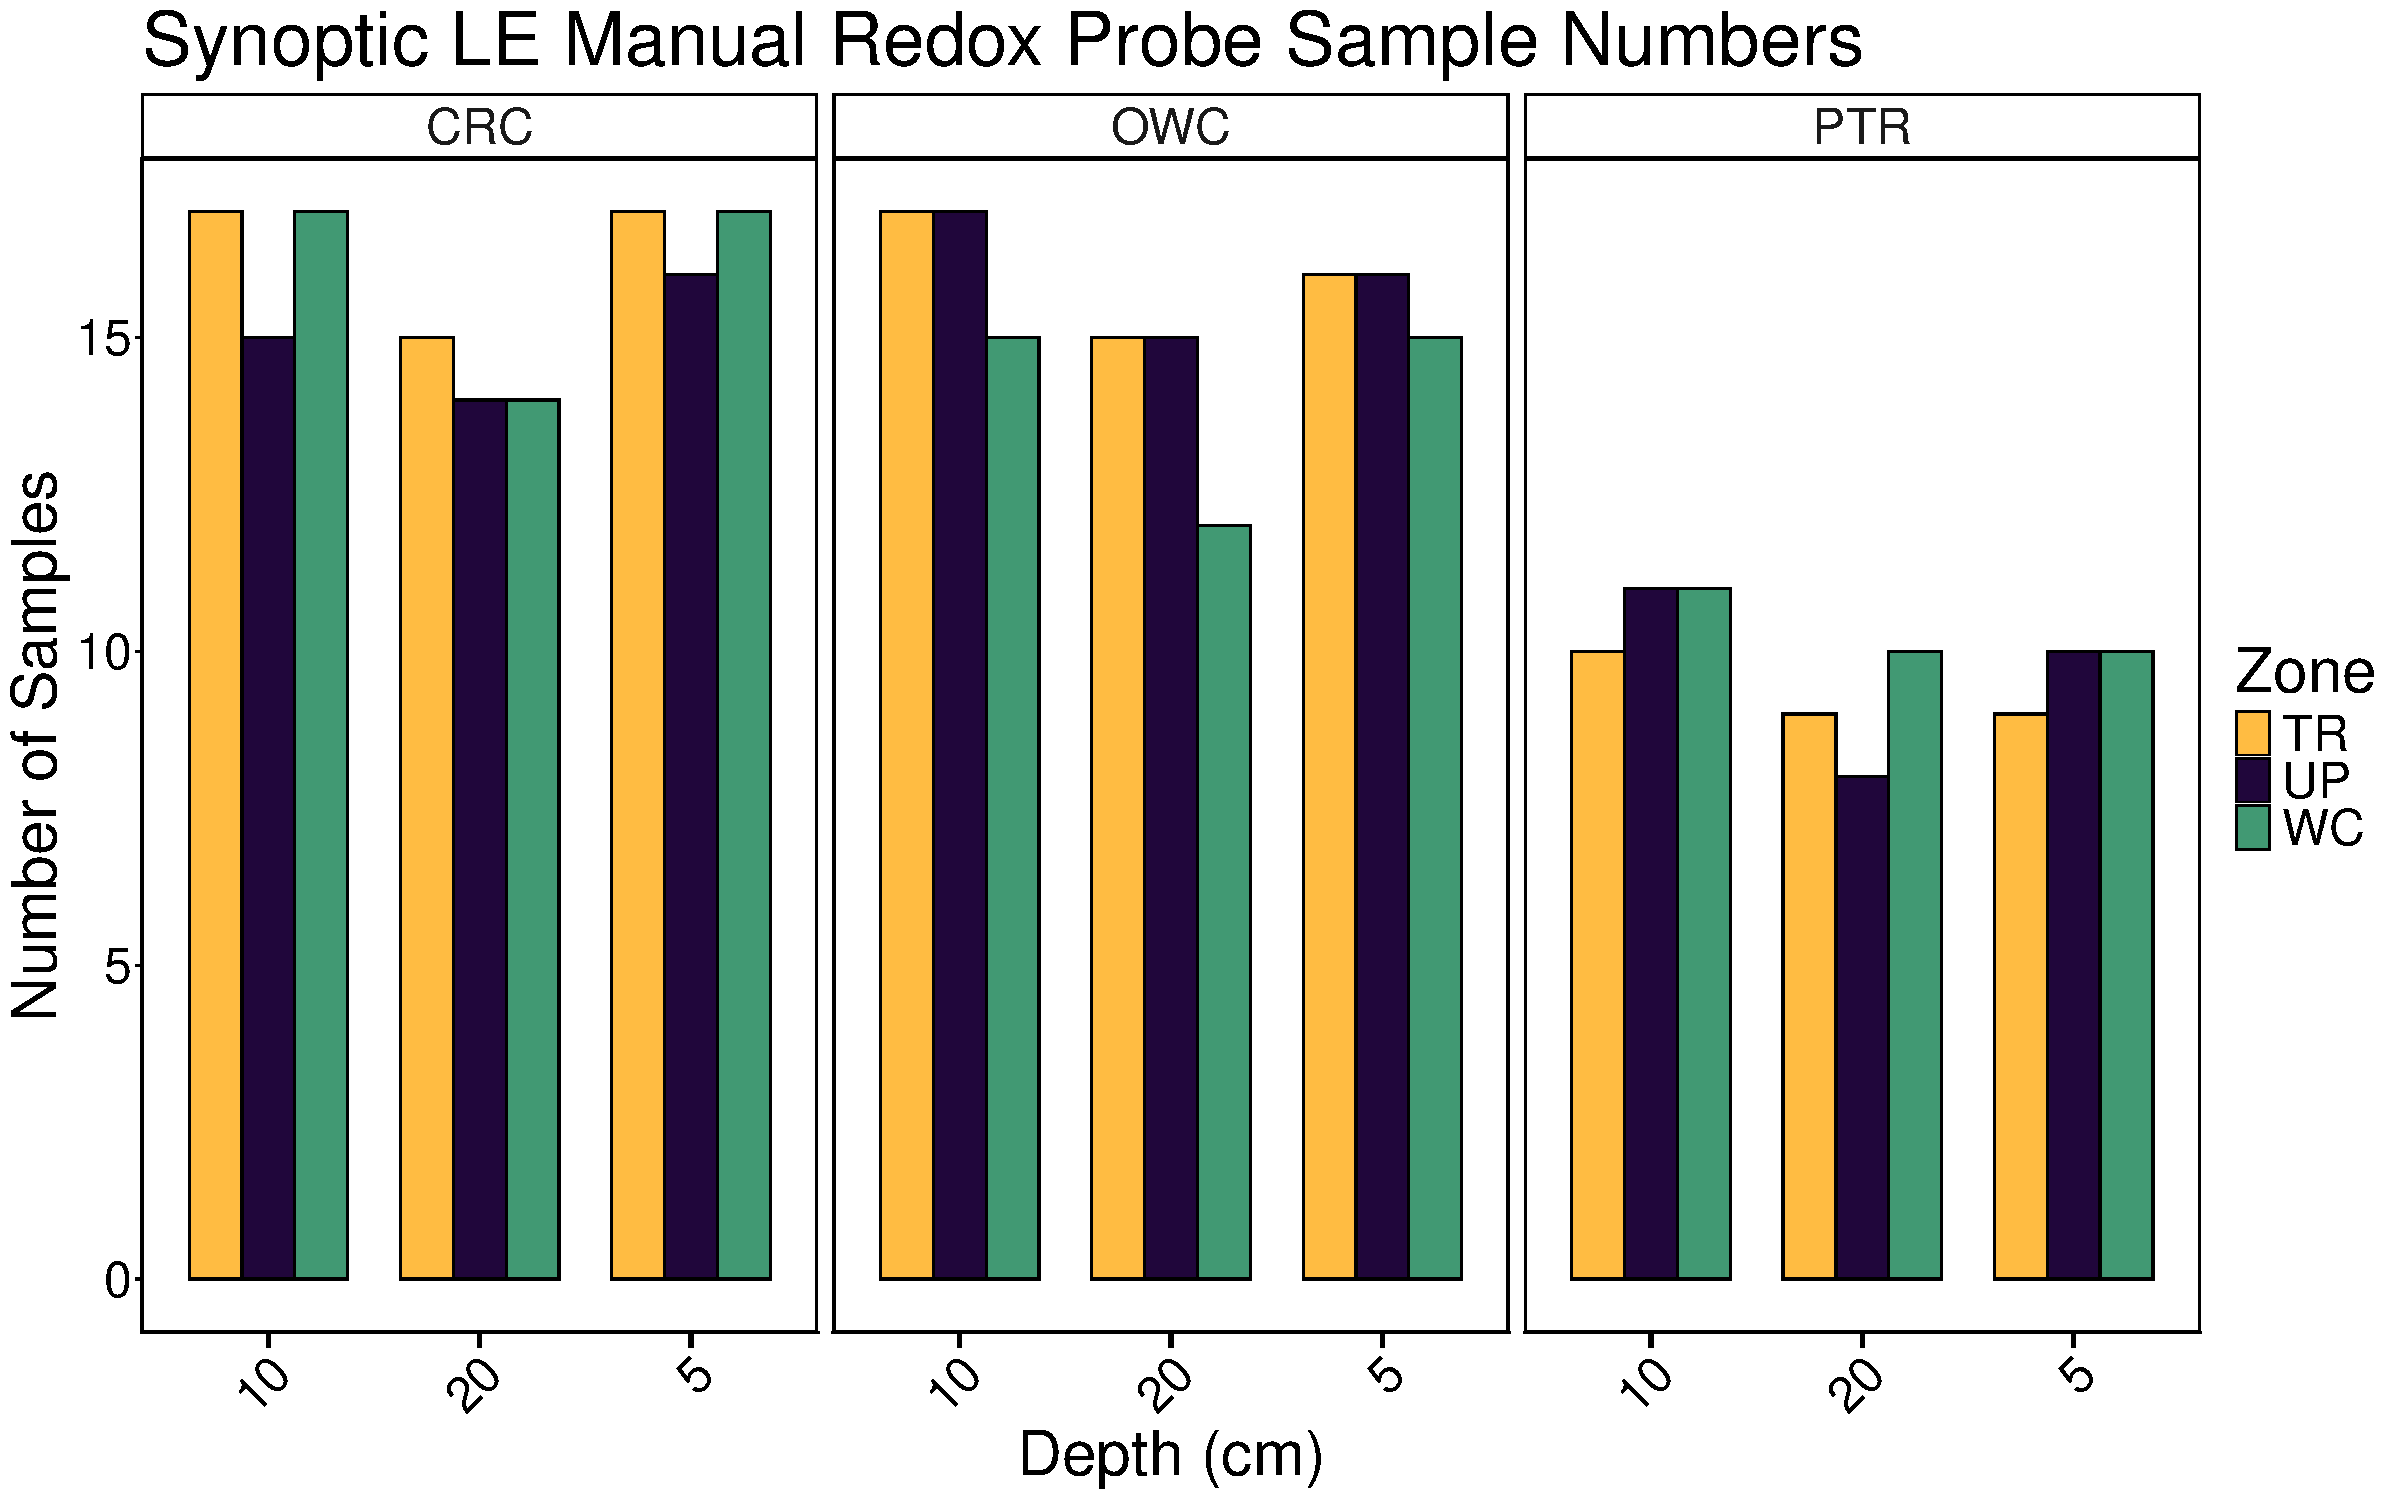
\includegraphics[keepaspectratio]{COMPASS_Synoptic_LE_Redox_Data_Processing_2022-2025_files/figure-pdf/Number of Samples Barplots-1.pdf}}




\end{document}
